% Nodal cubic y^2=x^3+x^2 (parametrised x=t^2-1, y=t(t^2-1)); the variety V(xz,yz) in R^3. Generated by a short script.
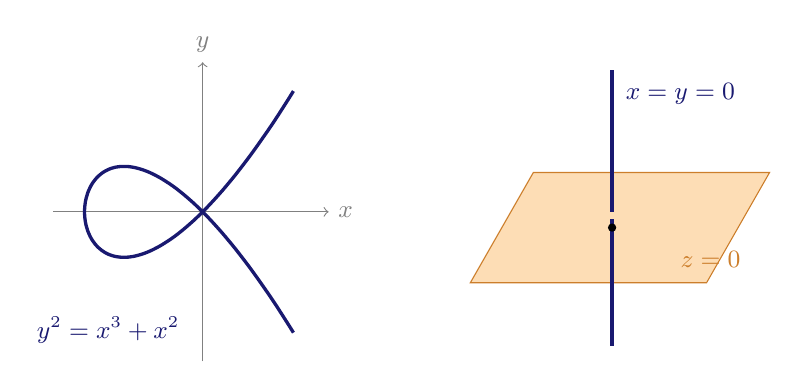
\begin{tikzpicture}[font=\small]
\draw[->,gray] (-1.9,0) -- (1.6,0) node[right] {$x$}; \draw[->,gray] (0,-1.9) -- (0,1.9) node[above] {$y$};
\draw[very thick,MidnightBlue] (1.153,-1.534) -- (1.087,-1.428) -- (1.022,-1.326) -- (0.958,-1.226) -- (0.895,-1.130) -- (0.832,-1.037) -- (0.770,-0.948) -- (0.709,-0.861) -- (0.649,-0.777) -- (0.590,-0.696) -- (0.531,-0.618) -- (0.474,-0.544) -- (0.417,-0.471) -- (0.361,-0.402) -- (0.306,-0.336) -- (0.252,-0.272) -- (0.198,-0.211) -- (0.145,-0.152) -- (0.094,-0.097) -- (0.043,-0.043) -- (-0.007,0.007) -- (-0.057,0.056) -- (-0.105,0.102) -- (-0.153,0.145) -- (-0.200,0.186) -- (-0.246,0.225) -- (-0.291,0.261) -- (-0.335,0.296) -- (-0.379,0.328) -- (-0.422,0.358) -- (-0.464,0.385) -- (-0.505,0.411) -- (-0.545,0.435) -- (-0.584,0.456) -- (-0.623,0.476) -- (-0.660,0.494) -- (-0.697,0.510) -- (-0.733,0.524) -- (-0.769,0.537) -- (-0.803,0.547) -- (-0.837,0.556) -- (-0.869,0.564) -- (-0.901,0.569) -- (-0.932,0.574) -- (-0.963,0.576) -- (-0.992,0.577) -- (-1.021,0.577) -- (-1.049,0.575) -- (-1.075,0.572) -- (-1.102,0.568) -- (-1.127,0.562) -- (-1.151,0.555) -- (-1.175,0.547) -- (-1.198,0.538) -- (-1.220,0.527) -- (-1.241,0.516) -- (-1.261,0.503) -- (-1.281,0.490) -- (-1.299,0.475) -- (-1.317,0.460) -- (-1.334,0.444) -- (-1.350,0.427) -- (-1.366,0.409) -- (-1.380,0.390) -- (-1.394,0.371) -- (-1.407,0.351) -- (-1.419,0.330) -- (-1.430,0.309) -- (-1.440,0.287) -- (-1.450,0.265) -- (-1.459,0.242) -- (-1.466,0.219) -- (-1.473,0.196) -- (-1.480,0.172) -- (-1.485,0.148) -- (-1.490,0.124) -- (-1.493,0.099) -- (-1.496,0.075) -- (-1.498,0.050) -- (-1.500,0.025) -- (-1.500,-0.000) -- (-1.500,-0.025) -- (-1.498,-0.050) -- (-1.496,-0.075) -- (-1.493,-0.099) -- (-1.490,-0.124) -- (-1.485,-0.148) -- (-1.480,-0.172) -- (-1.473,-0.196) -- (-1.466,-0.219) -- (-1.459,-0.242) -- (-1.450,-0.265) -- (-1.440,-0.287) -- (-1.430,-0.309) -- (-1.419,-0.330) -- (-1.407,-0.351) -- (-1.394,-0.371) -- (-1.380,-0.390) -- (-1.366,-0.409) -- (-1.350,-0.427) -- (-1.334,-0.444) -- (-1.317,-0.460) -- (-1.299,-0.475) -- (-1.281,-0.490) -- (-1.261,-0.503) -- (-1.241,-0.516) -- (-1.220,-0.527) -- (-1.198,-0.538) -- (-1.175,-0.547) -- (-1.151,-0.555) -- (-1.127,-0.562) -- (-1.102,-0.568) -- (-1.075,-0.572) -- (-1.049,-0.575) -- (-1.021,-0.577) -- (-0.992,-0.577) -- (-0.963,-0.576) -- (-0.932,-0.574) -- (-0.901,-0.569) -- (-0.869,-0.564) -- (-0.837,-0.556) -- (-0.803,-0.547) -- (-0.769,-0.537) -- (-0.733,-0.524) -- (-0.697,-0.510) -- (-0.660,-0.494) -- (-0.623,-0.476) -- (-0.584,-0.456) -- (-0.545,-0.435) -- (-0.505,-0.411) -- (-0.464,-0.385) -- (-0.422,-0.358) -- (-0.379,-0.328) -- (-0.335,-0.296) -- (-0.291,-0.261) -- (-0.246,-0.225) -- (-0.200,-0.186) -- (-0.153,-0.145) -- (-0.105,-0.102) -- (-0.057,-0.056) -- (-0.007,-0.007) -- (0.043,0.043) -- (0.094,0.097) -- (0.145,0.152) -- (0.198,0.211) -- (0.252,0.272) -- (0.306,0.336) -- (0.361,0.402) -- (0.417,0.471) -- (0.474,0.544) -- (0.531,0.618) -- (0.590,0.696) -- (0.649,0.777) -- (0.709,0.861) -- (0.770,0.948) -- (0.832,1.037) -- (0.895,1.130) -- (0.958,1.226) -- (1.022,1.326) -- (1.087,1.428) -- (1.153,1.534);
\node[MidnightBlue] at (-1.2,-1.5) {$y^2=x^3+x^2$};
\begin{scope}[xshift=5.2cm]
\fill[BurntOrange!25] (-1.8,-0.9) -- (1.2,-0.9) -- (2.0,0.5) -- (-1.0,0.5) -- cycle;
\draw[BurntOrange!80!black] (-1.8,-0.9) -- (1.2,-0.9) -- (2.0,0.5) -- (-1.0,0.5) -- cycle;
\draw[very thick,MidnightBlue] (0,-0.2) -- (0,-1.7); \draw[very thick,MidnightBlue,dashed] (0,-0.2) -- (0,0.0); \draw[very thick,MidnightBlue] (0,0.0) -- (0,1.8);
\fill (0,-0.2) circle (1.5pt);
\node[BurntOrange!80!black] at (1.25,-0.6) {$z=0$}; \node[MidnightBlue,right] at (0.05,1.5) {$x=y=0$};
\end{scope}
\end{tikzpicture}
